\subsection{Исследование RC-цепи}

\subsubsection{Схема исследуемой цепи}
На рисунке 1.1 представлена схема замещения источника электрической энергии постоянного тока и нагрузки, созданная в приложении LTspice.

% \begin{figure}[H]
% 	\centering
% 	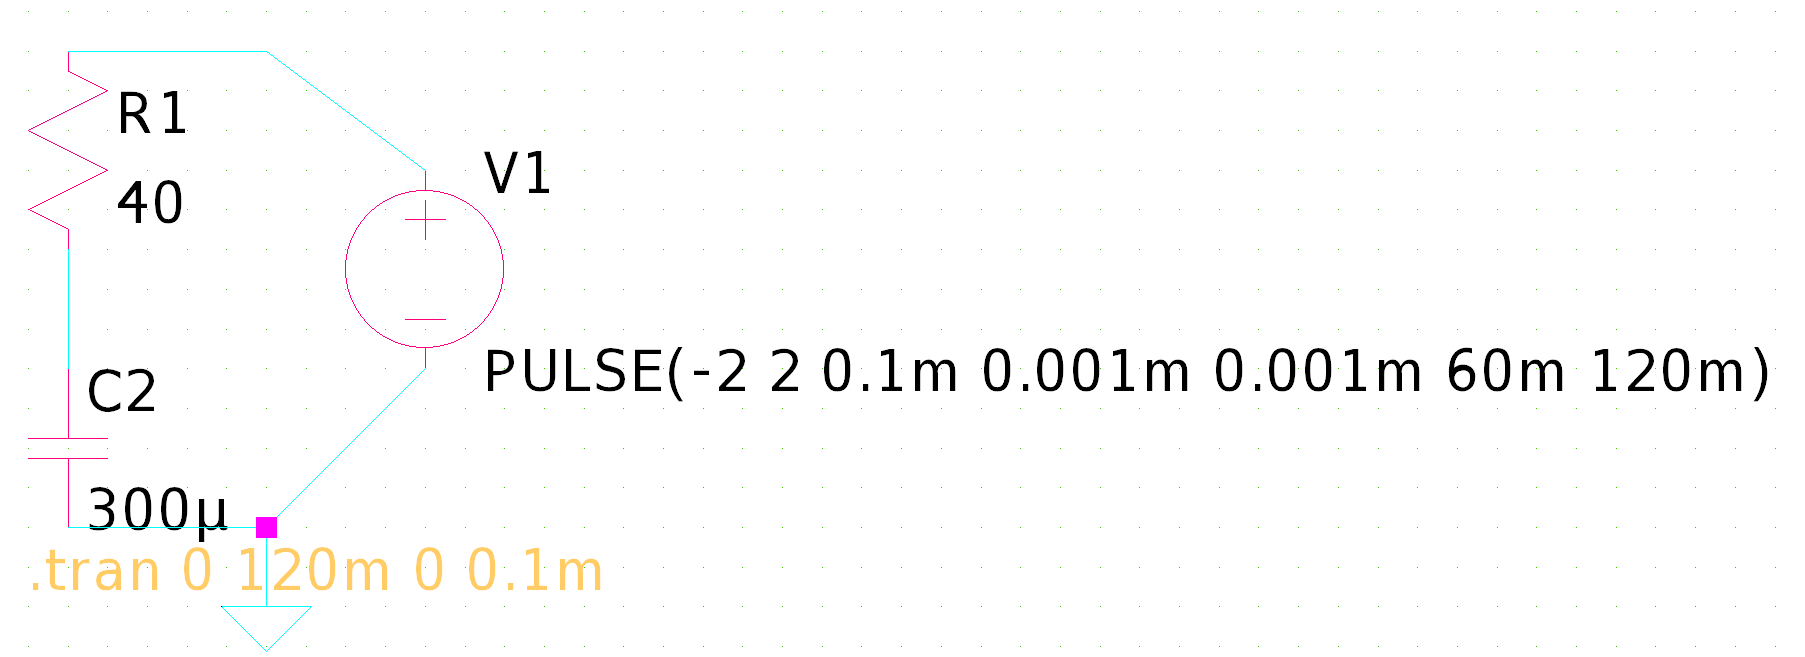
\includegraphics[width=0.6\textwidth]{rc-schema.png} % Make sure the path to the image is correct
% 	\caption{Схема замещения источника электрической энергии в LTspice.}
% \end{figure}

\subsubsection{Расчётные формулы и расчёты}

\subsubsection{Графики переходных процессов}

\subsubsection{Таблица результатов 4.2}

\subsection{Исследование RL-цепи}

\subsubsection{Схема исследуемой цепи}
На рисунке 1.1 представлена схема замещения источника электрической энергии постоянного тока и нагрузки, созданная в приложении LTspice.

% \begin{figure}[H]
% 	\centering
% 	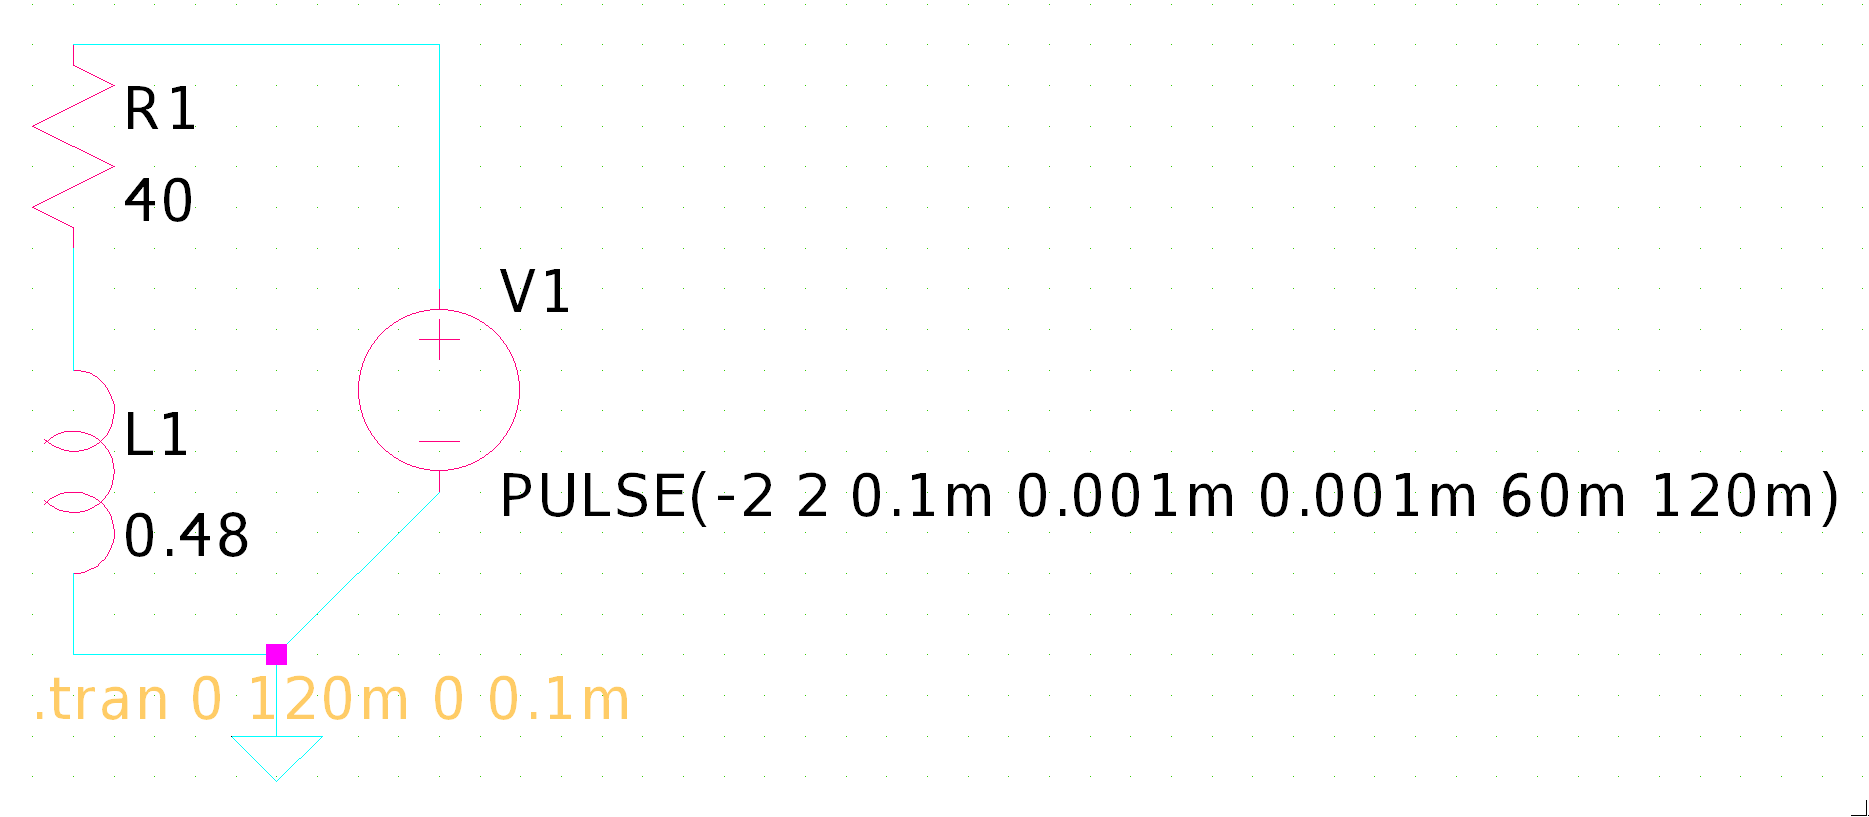
\includegraphics[width=0.6\textwidth]{rl-schema.png} % Make sure the path to the image is correct
% 	\caption{Схема замещения источника электрической энергии в LTspice.}
% \end{figure}

\subsubsection{Расчётные формулы и расчёты}

\subsubsection{Графики переходных процессов}

\subsubsection{Таблица результатов 4.3}

\subsection{Выводы по первой части}
